\begin{figure}[t]
\centering
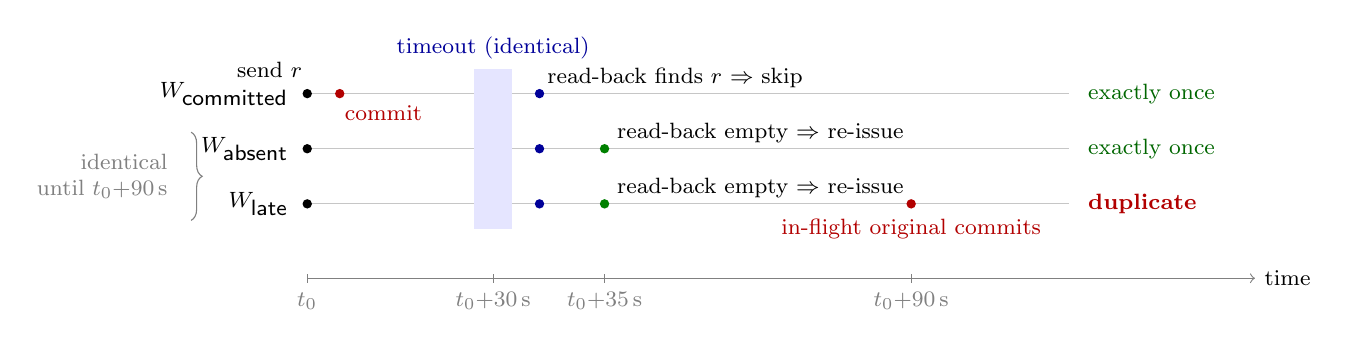
\begin{tikzpicture}[x=1.18cm,y=0.7cm,font=\footnotesize,
  ev/.style={circle,fill=black,inner sep=1.2pt},
  lbl/.style={align=left,inner sep=1pt}]
  \draw[->,gray] (0,-0.35) -- (10.2,-0.35) node[right,black]{time};
  \foreach \x/\t in {0/$t_0$,2/$t_0{+}30$\,s,3.2/$t_0{+}35$\,s,6.5/$t_0{+}90$\,s} {
    \draw[gray] (\x,-0.43) -- (\x,-0.27); \node[below,gray] at (\x,-0.43) {\t};
  }
  \foreach \y/\n in {3/$W_{\textsf{committed}}$,2/$W_{\textsf{absent}}$,1/$W_{\textsf{late}}$} {
    \draw[gray!45] (0,\y) -- (8.2,\y); \node[anchor=east] at (-0.1,\y) {\n}; \node[ev] at (0,\y) {};
  }
  \node[above left] at (0.05,3.12) {send $r$};
  % commits
  \node[ev,fill=red!70!black] at (0.35,3) {}; \node[below right,red!70!black] at (0.3,2.95) {commit};
  \node[ev,fill=red!70!black] at (6.5,1) {}; \node[below,red!70!black] at (6.5,0.9) {in-flight original commits};
  % the timeout, identical everywhere
  \fill[blue!10] (1.8,0.55) rectangle (2.2,3.45);
  \node[above,blue!60!black] at (2,3.45) {timeout (identical)};
  % read-back
  \foreach \y in {3,2,1} { \node[ev,fill=blue!60!black] at (2.5,\y) {}; }
  \node[lbl,right] at (2.55,3.28) {read-back finds $r$ $\Rightarrow$ skip};
  \node[lbl,right] at (3.3,2.28) {read-back empty $\Rightarrow$ re-issue};
  \node[lbl,right] at (3.3,1.28) {read-back empty $\Rightarrow$ re-issue};
  \node[ev,fill=green!50!black] at (3.2,2) {}; \node[ev,fill=green!50!black] at (3.2,1) {};
  % outcomes
  \node[right,green!40!black] at (8.3,3) {exactly once};
  \node[right,green!40!black] at (8.3,2) {exactly once};
  \node[right,red!70!black] at (8.3,1) {\textbf{duplicate}};
  % equivalence bracket
  \draw[decorate,decoration={brace,amplitude=4pt,mirror},gray] (-1.25,0.7) -- (-1.25,2.3)
    node[midway,left=5pt,align=right,gray]{identical\\until $t_0{+}90$\,s};
\end{tikzpicture}
\caption{Why verification is not enough. $W_{\textsf{absent}}$ and $W_{\textsf{late}}$ produce identical
observations---a timeout and then an empty read-back---until the in-flight original commits, so
verify-then-retry re-issues in both and duplicates in $W_{\textsf{late}}$ (Proposition~\ref{prop:late}). If the
re-issue reuses the original's idempotency key, the late original becomes a no-op in every world
(Proposition~\ref{prop:keys}).}
\label{fig:timeline}
\end{figure}
